% !TEX root = ./document.tex

\documentclass[11pt]{article}

\usepackage{mystyle}
\usepackage{myvars}

%-----------------------------

\begin{document}

  \maketitle

  %-----------------------------
  %  TEXT
  %-----------------------------

  \section{Contexto y Conjunto de Datos}

    \paragraph{}
    En este trabajo se va a realizar un estudio acerca de la diferencia de medias sobre el conjunto de datos \texttt{painkillers}, el cual se refiere a un experimento sobre \emph{Analgésicos Infantiles}. Para ello, se utilizará la técnica de \emph{Análisis de la Varianza (ANOVA)}. Una contextualización más detallada del experimento se describe a partir del siguiente enunciado:

    \paragraph{}
    \say{El departamento de pediatría de un hospital desea analizar la eficacia de cuatro analgésicos infantiles ante las cefaleas. Para ello, realiza un experimento en el que se seleccionan aleatoriamente cinco grupos de cuatro pacientes, de manera que en cada grupo se da un cefalea distinto. A continuación se suministra, también de forma aleatoria, cada analgésico a uno de los pacientes de cada grupo, y se observa el tiempo de remisión de la cefalea, en minutos. Se registran los datos siguientes, en cada uno de los cinco grupos (\texttt{tiempo de remisión}, \texttt{analgésico} y \texttt{cefalea}).}

  \section{Cuestiones}

    \paragraph{}
    En esta sección se incluyen una serie de cuestiones que serán resueltas mediante el estudio del conjunto de datos a partir de la técnica \emph{ANOVA}.

    \subsection{Estudia el tipo de diseño adecuado para esta situación, e identifica las variables, factores y parámetros}

      \paragraph{}
      Tras analizar el contexto del experimento, se sabe que la variable respuesta $Y$ que se utilizará para el \emph{análisis de la varianza} es \texttt{tiempo de remisión}, dado que es la que se utiliza para cuantificar la calidad del tratamiento. En cuanto a las variables a partir de las cuales se pretende explicar el \texttt{tiempo de remisión}, estas son el \texttt{analgésico} y el \texttt{cefalea}.

      \paragraph{}
      Sin embargo, estas no han sido seleccionadas de la misma manera, dado que tal y como se indica en el enunciado, se han fijado $4$ muestras de \emph{a priori} $5$ \texttt{tipos de cefalea}, sobre los cuales aplicar los $4$ tipos de \texttt{analgésico}. Por tanto, podemos interpretar dicha situación diciendo que el factor \texttt{tipos de cefalea} representa un \textbf{bloque} (que denotaremos por $B_\beta$ siendo $\beta \in \{1,2,3,4,5\}$ el identificador de cada uno de los niveles del bloque), y asumiento que el factor \texttt{analgésico} representa un \textbf{tratamiento} (que denotaremos por $T_\alpha $ siendo $\alpha \in \{A, B, C, D\}$ el identificador de cada uno de los niveles del tratamiento).

      \begin{align}
      \label{eq:1f1b_model}
        Y_{ij} = \mu + T_\alpha + B_\beta + \epsilon_ij
      \end{align}

      \paragraph{}
      Por dichas razones, utilizaremos el modelo de \emph{1 factor + 1 bloque}, el cual se muestra en la ecuación \eqref{eq:1f1b_model}. A este modelo se le ha añadido además la componente $\epsilon_ij$, que representa el error aleatorio y sigue una distribución $N(0, \sigma^2)$, asumiendo que $\sigma^2$ es la misma para todas las observaciones.

      \paragraph{}
      [TODO]

      \begin{figure}[H]
        \centering
        \begin{subfigure}{.5\textwidth}
          \centering
          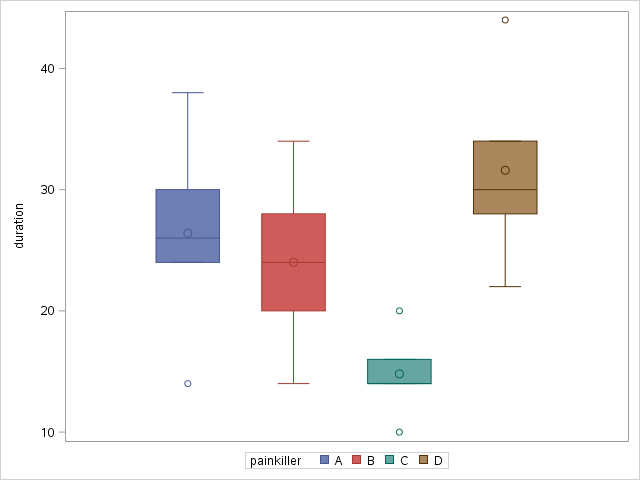
\includegraphics[width=\linewidth]{box-plot-analgesico}
          \caption{\texttt{analgésico}}
          \label{fig:sub1}
        \end{subfigure}%
        \begin{subfigure}{.5\textwidth}
          \centering
          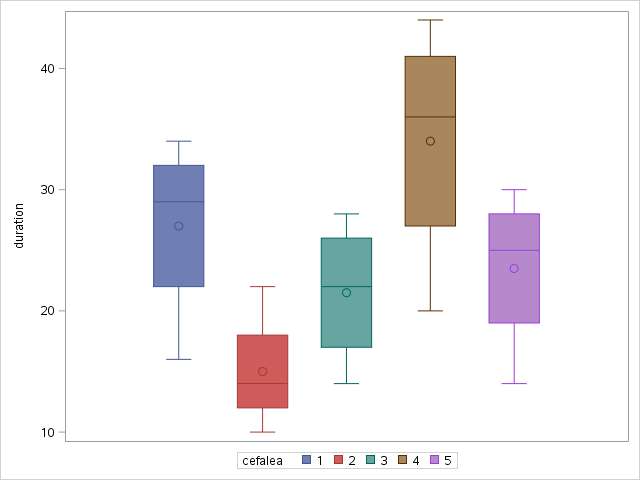
\includegraphics[width=\linewidth]{box-plot-cefalea}
          \caption{\texttt{cefalea}}
          \label{fig:sub2}
        \end{subfigure}
        \caption{Diagramas de cajas}
        \label{fig:test}
      \end{figure}


    \subsection{?`Es adecuado usar las cefaleas como bloques?. ?`Existen diferencias significativas entre los tiempos de remisión de las cefaleas para los distintos analgésicos?}

      \paragraph{}
      [TODO]

      \begin{figure}[H]
        \centering
        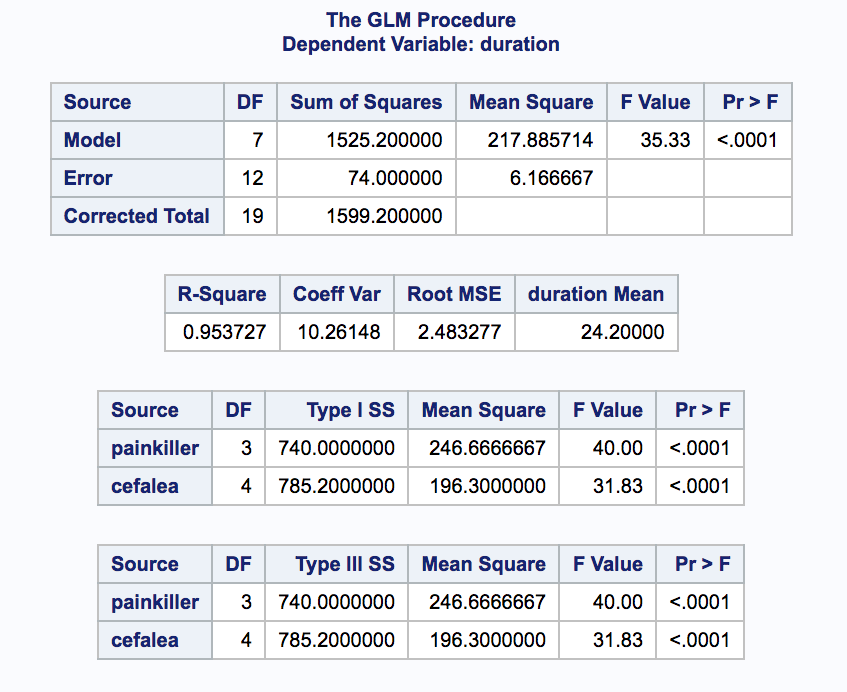
\includegraphics[width=.5\textwidth]{blocks-anova}
        \caption{}
        \label{}
      \end{figure}

    \subsection{Estudia gráficamente la existencia de interacción entre analgésico y cefalea.}

      \paragraph{}
      [TODO]

      \begin{figure}[H]
        \centering
        \begin{subfigure}{.5\textwidth}
          \centering
          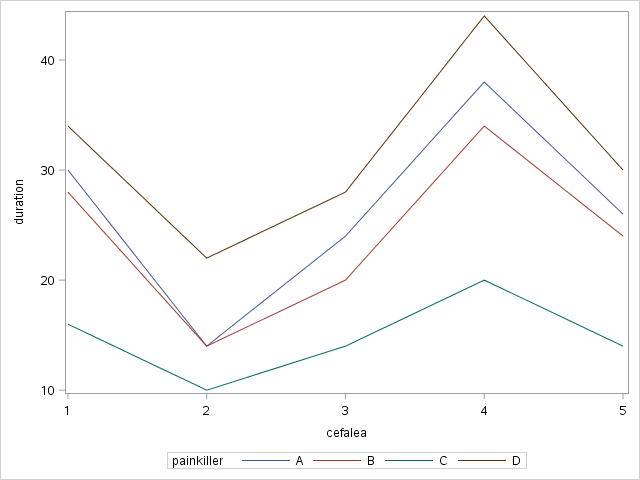
\includegraphics[width=\linewidth]{interaction-analgesico}
          \caption{\texttt{analgésico}}
          \label{fig:sub1}
        \end{subfigure}%
        \begin{subfigure}{.5\textwidth}
          \centering
          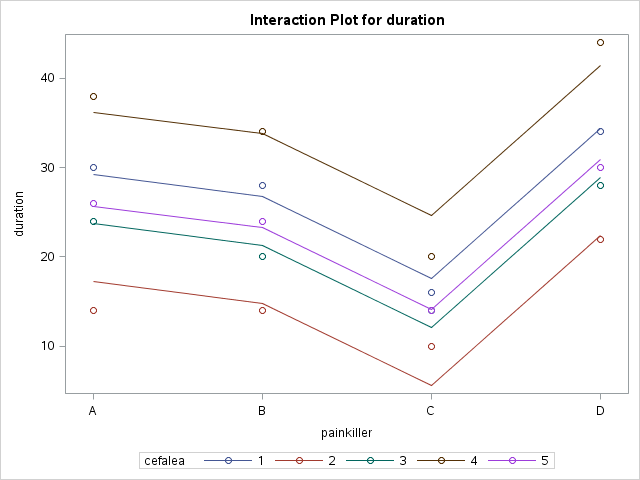
\includegraphics[width=\linewidth]{interaction-cefalea}
          \caption{\texttt{cefalea}}
          \label{fig:sub2}
        \end{subfigure}
        \caption{Diagramas de Interacción}
        \label{fig:test}
      \end{figure}


    \subsection{Determina mediante comparaciones múltiples cuál de los analgésicos es más eficaz.}

      \paragraph{}
      [TODO]

      \begin{figure}[H]
        \centering
        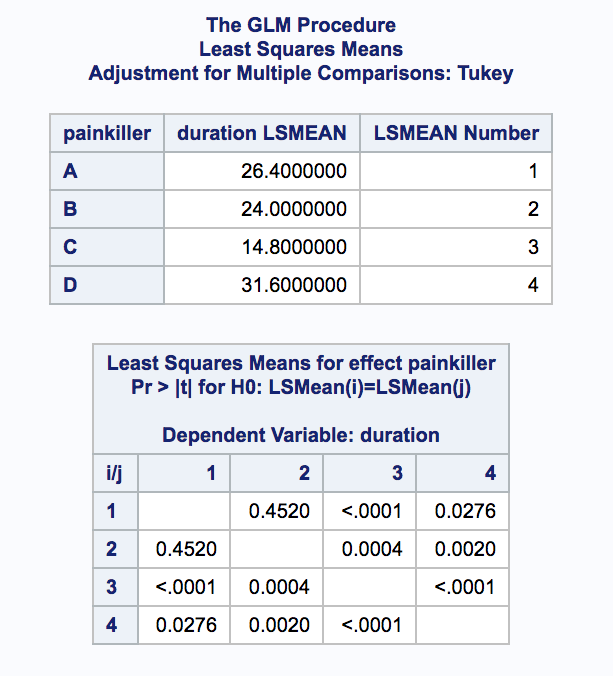
\includegraphics[width=.5\textwidth]{tukey-test}
        \caption{}
        \label{}
      \end{figure}

      \begin{figure}[H]
        \centering
        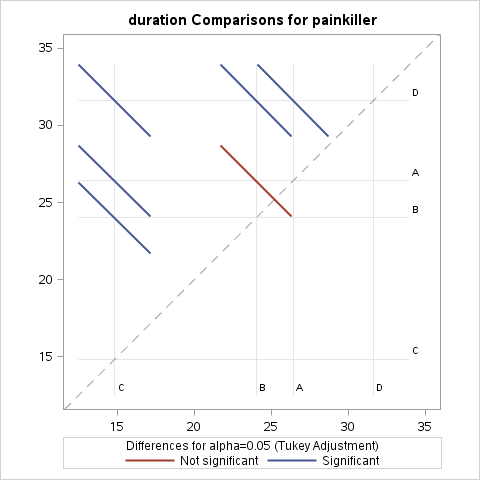
\includegraphics[width=.5\textwidth]{plot-tukey}
        \caption{}
        \label{}
      \end{figure}

    \subsection{Suponiendo que el analgésico A es un placebo, realiza el test de Dunnett}

      \paragraph{}
      [TODO]


      \begin{figure}[H]
        \centering
        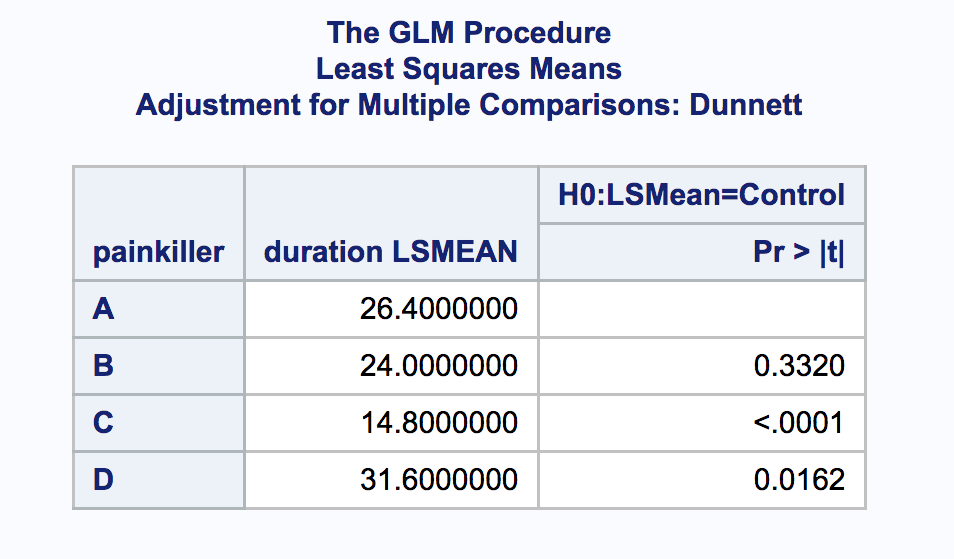
\includegraphics[width=.5\textwidth]{dunnet-test}
        \caption{}
        \label{}
      \end{figure}

      \begin{figure}[H]
        \centering
        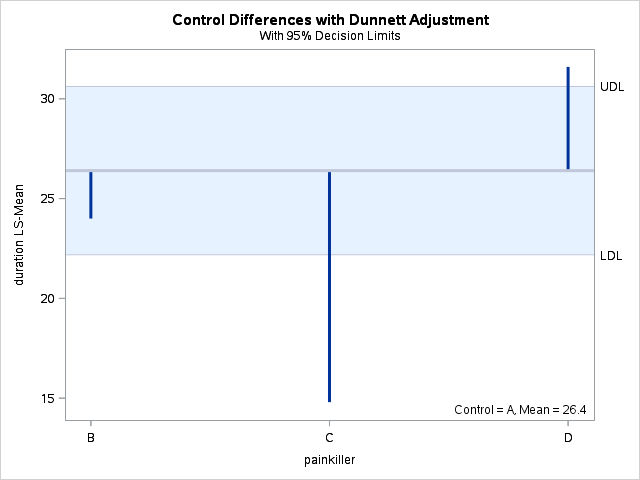
\includegraphics[width=.5\textwidth]{plot-dunnet}
        \caption{}
        \label{}
      \end{figure}


    \subsection{Haz un análisis gráfico de los residuos.}

      \paragraph{}
      [TODO]

      \begin{figure}[H]
        \centering
        \begin{subfigure}{.5\textwidth}
          \centering
          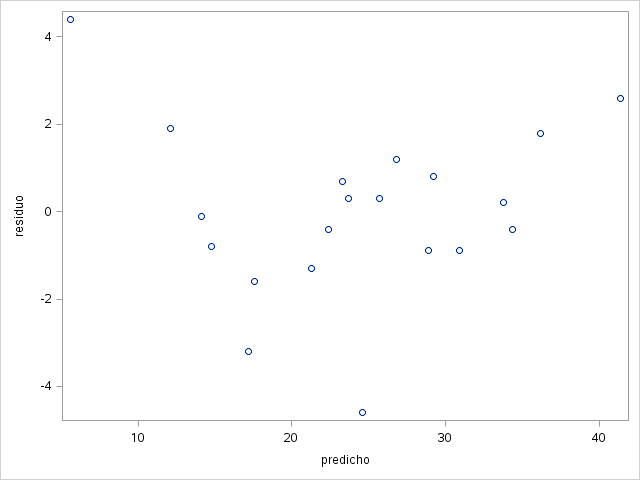
\includegraphics[width=\linewidth]{residuos}
          \caption{Resodios Estándar}
          \label{fig:sub1}
        \end{subfigure}%
        \begin{subfigure}{.5\textwidth}
          \centering
          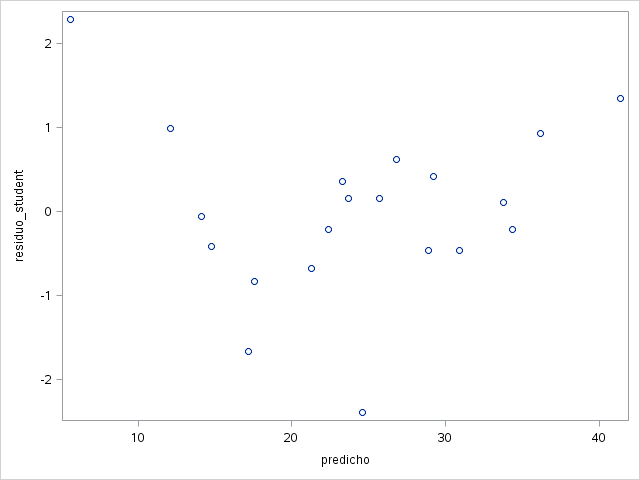
\includegraphics[width=\linewidth]{residuos-student}
          \caption{Residuos Studentizados}
          \label{fig:sub2}
        \end{subfigure}
        \caption{Diagramas de Residuos}
        \label{fig:test}
      \end{figure}

    \subsection{Si los analgésicos se hubieran elegido al azar entre todos los existentes, plantea el modelo adecuado y estima las componentes de la varianza.}

      \paragraph{}
      [TODO]


      \begin{figure}[H]
        \centering
        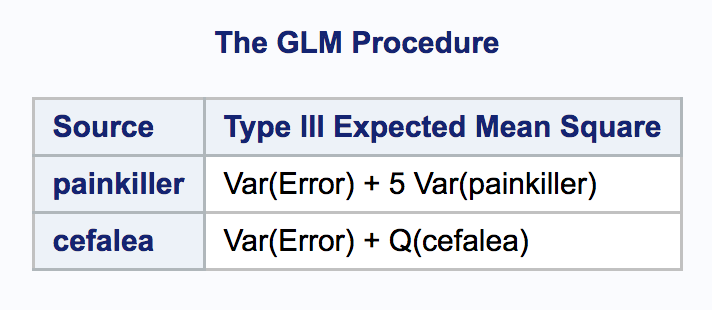
\includegraphics[width=.3\textwidth]{random-var}
        \caption{}
        \label{}
      \end{figure}


      \begin{figure}[H]
        \centering
        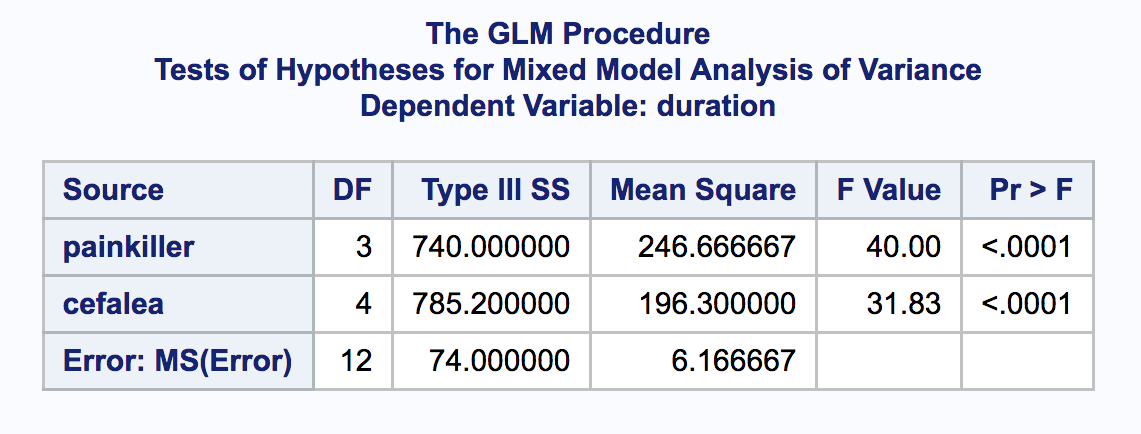
\includegraphics[width=.5\textwidth]{random-anova}
        \caption{}
        \label{}
      \end{figure}


    \subsection{Plantea el modelo como diseño unifactorial completamente aleatorizado y compara los resultados.}

      \paragraph{}
      [TODO]

      \begin{figure}[H]
        \centering
        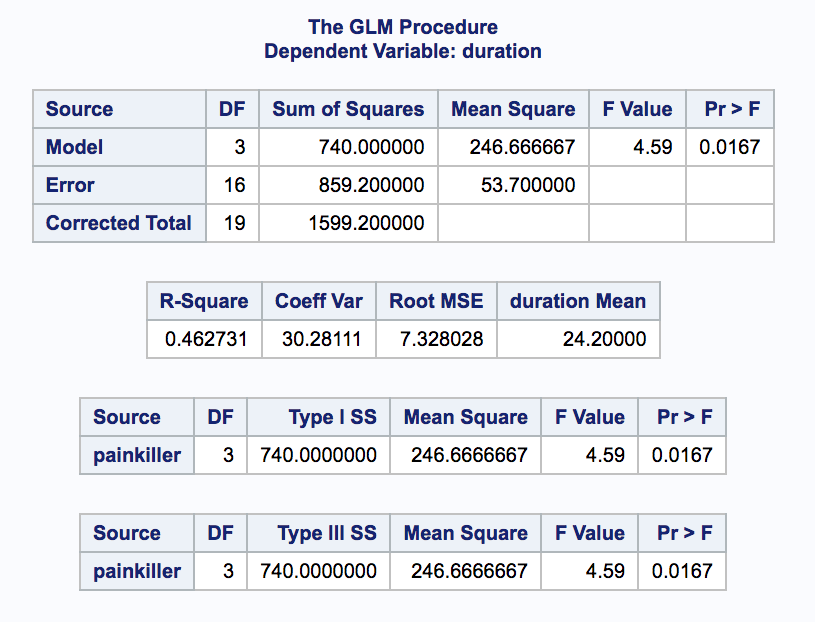
\includegraphics[width=.5\textwidth]{simple-anova}
        \caption{}
        \label{}
      \end{figure}

  \section{Código Fuente}

    \paragraph{}
    En esta sección se incluyen los distintos procedimientos de código \emph{SAS} utilizados para la realización de este trabajo.

    \begin{figure}[H]
      \centering
      \begin{minted}[frame=single,framesep=5pt]{sas}
data painkillers;
  input duration painkiller$ cefalea;
  datalines;
  30 A 1
  28 B 1
  16 C 1
  34 D 1
  14 A 2
  14 B 2
  10 C 2
  22 D 2
  24 A 3
  20 B 3
  14 C 3
  28 D 3
  38 A 4
  34 B 4
  20 C 4
  44 D 4
  26 A 5
  24 B 5
  14 C 5
  30 D 5
;
run;
proc print data=painkillers;
run;
      \end{minted}
      \caption{\emph{Código SAS:} Lectura del conjunto de datos.}
      \label{code:sas_1}
    \end{figure}

    \begin{figure}[H]
      \centering
      \begin{minted}[frame=single,framesep=5pt]{sas}

proc sgplot data=painkillers;
  vbox duration / group=painkiller;
run;

proc sgplot data=painkillers;
  vbox duration /group=cefalea;
run;
      \end{minted}
      \caption{\emph{Código SAS:} Generación de los diagramas de cajas.}
      \label{code:sas_2}
    \end{figure}

    \begin{figure}[H]
      \centering
      \begin{minted}[frame=single,framesep=5pt]{sas}
proc glm data=painkillers;
  *class cefalea painkiller;
  class painkiller cefalea;
  model duration=painkiller cefalea ;
  lsmeans painkiller / adjust=tukey;
  lsmeans painkiller / adjust=dunnett;
  random painkiller / test;
  output out=soluc P=predicho R=residuo student=residuo_student;
run;
      \end{minted}
      \caption{\emph{Código SAS:} Realización de ANOVA por bloques.}
      \label{code:sas_3}
    \end{figure}

    \begin{figure}[H]
      \centering
      \begin{minted}[frame=single,framesep=5pt]{sas}
proc sgplot data=soluc;
  scatter y=residuo x=predicho;
run;

proc sgplot data=soluc;
  scatter y=residuo_student x=predicho;
run;
      \end{minted}
      \caption{\emph{Código SAS:} Generación de diagramas de residuos.}
      \label{code:sas_4}
    \end{figure}
    \begin{figure}[H]
      \centering
      \begin{minted}[frame=single,framesep=5pt]{sas}
proc glm data=painkillers;
  class painkiller;
  model duration=painkiller;
run;
      \end{minted}
      \caption{\emph{Código SAS:} Realización de ANOVA completamente aleatorizado.}
      \label{code:sas_5}
    \end{figure}
  %-----------------------------
  %  Bibliographic references
  %-----------------------------

  \nocite{rano2017}
  \nocite{sas}

  \bibliographystyle{acm}
  \bibliography{bib}

\end{document}
